\section{The System Architecture}

\subsection{Description of the Architecture and Tools used}
As is shown in Figure \ref{fig:archi}, our system has four main steps : Feature Extraction, Sampling, Clustering and Visualization. The tools we use includes Amazon Elastic MapReduce\cite{EMR}, Scikit-learn\cite{sklearn} library and Google Map API\cite{GoogleMap}. The four steps are illustrated in details in the followling part.
\begin{figure}[htbp]
				\centering
				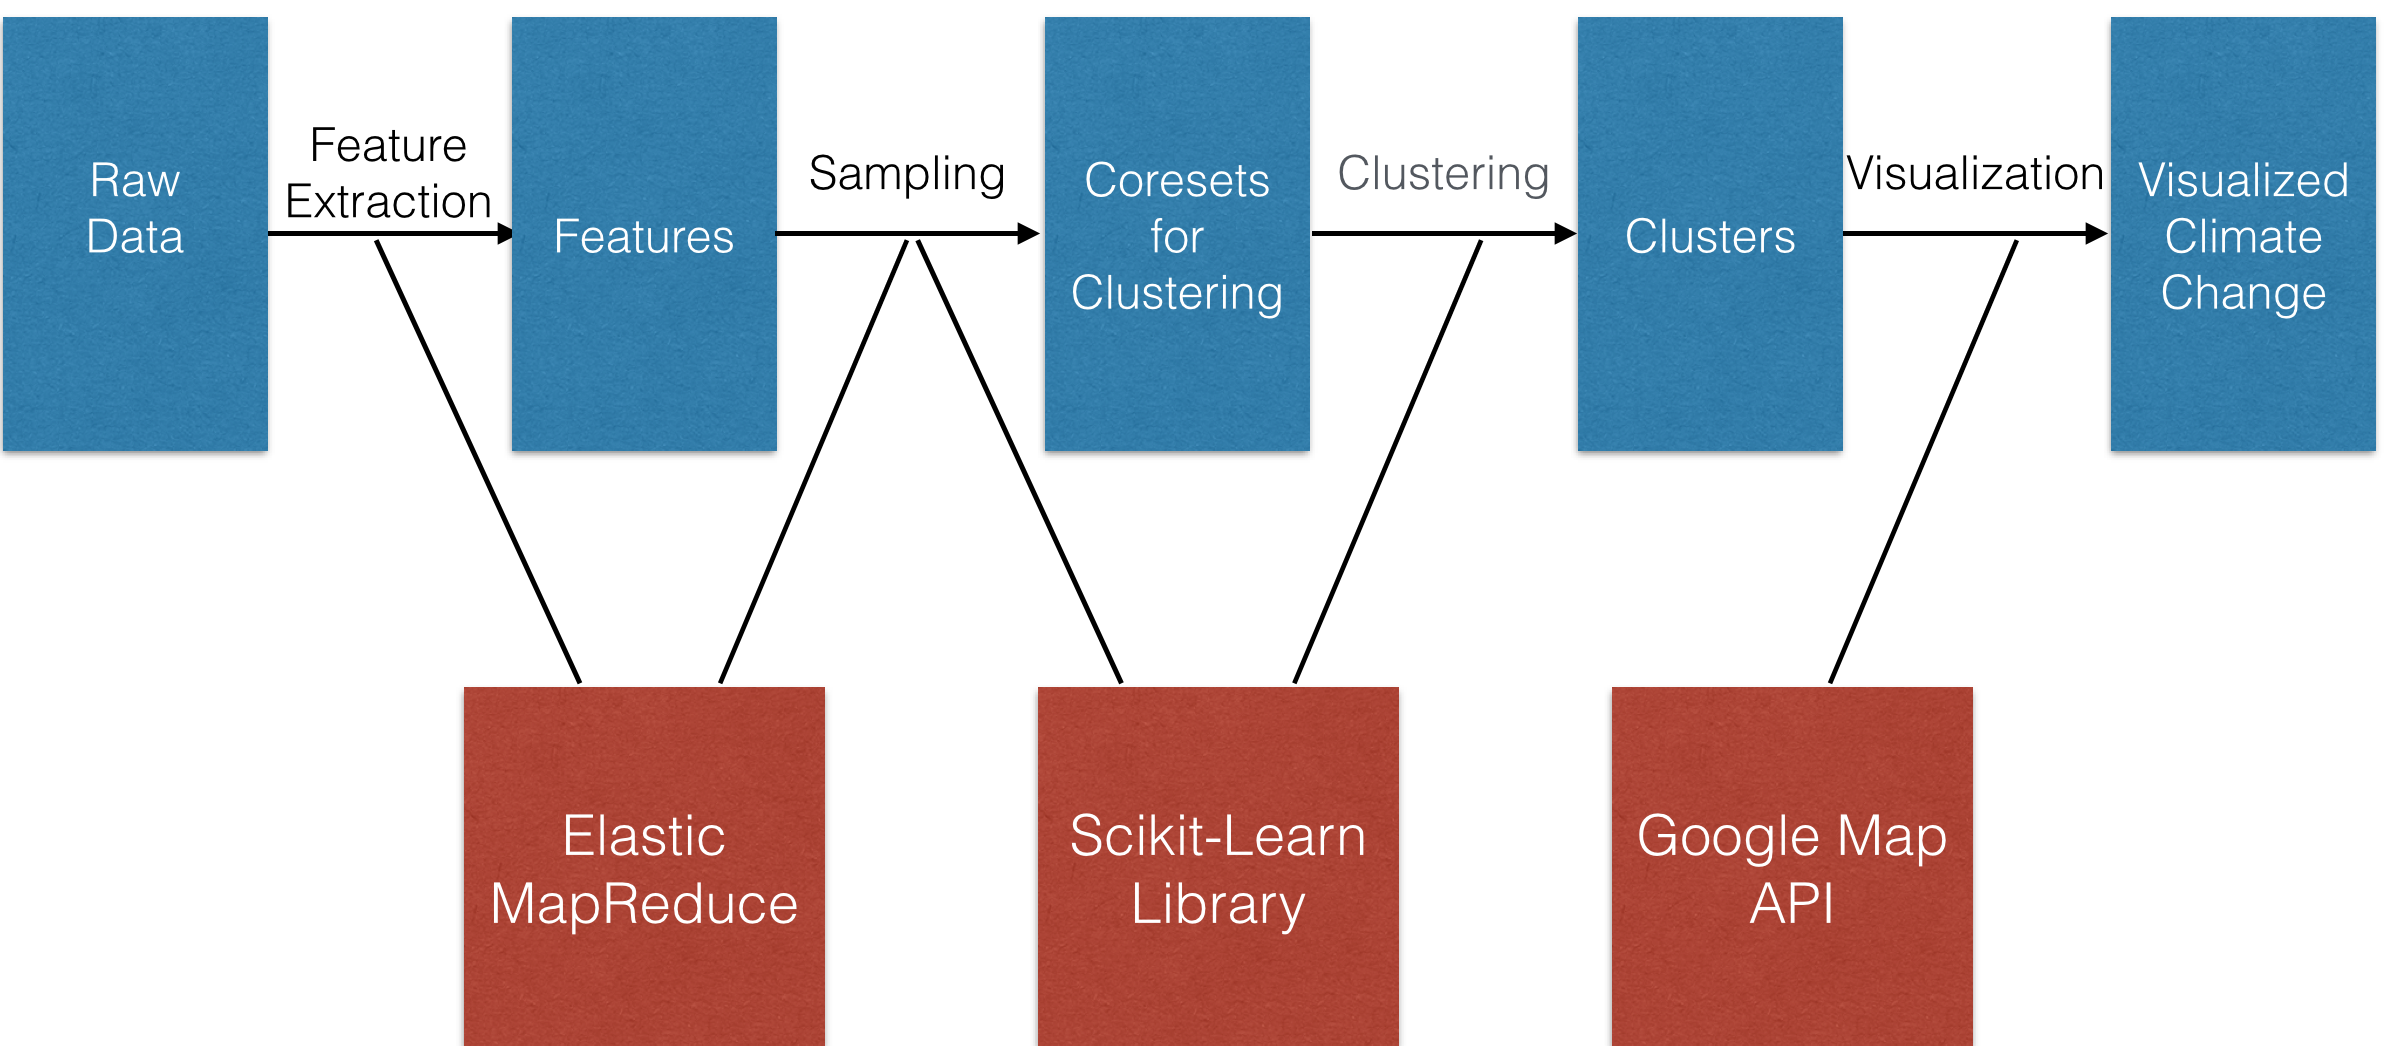
\includegraphics[width=0.9\textwidth]{figure/Architecture.png}
				\caption{Architecture of our system}
				\label{fig:archi}
 \end{figure}
 
\subsubsection{Feature Extraction}
The raw data includes the climate data from 1763 to 2014, the total volume of raw data is about 100 Gigabytes, which is too big to fit in the memory. So we use Amazon Elastic MapReduce to calculate features. We use the same features setting with the previous milestone. The feature extraction consists of 3 sub-steps, including calculating features for existing data, filling in the missing value using the mean value of the feature value of all other existing data and normalizing data. Each of these sub-step is done by a map-reduce task bacause of the huge volume of data. Through feature extraction, we get about 300 million 60-dimentional data points.

\subsubsection{Sampling}
We want to use all data points to run clustering. However, we use the k-means function in the scikit-learn library to compute clusters. It is impossible for that k-means function to run on 300 million of data points. We have two choices of handling this. One is to write a parrallel k-means function that can run on Amazon EMR, the other one is to sample these data points so that the sample points are able to represent all the data points with the minimum loss of information. We choose the second approach and use coreset for k-means clustering. The coreset is a set of data points that is used to run the weighted k-means clustering. Each point in the coreset represents some oringinal data points that are near to it. These data points are assigned the same label as the point in the coreset. The coreset sampling is done by an iterative step, where in each step, we uniformly sample some data points, calculate distance to the nearest point in the sampling set for every data point, remove data points whose distance to the nearest point in the sampling set are below median. Iterate this step until the number of remained data points is smaller than a pre-defined number and we get a coreset sampling of data.

\subsubsection{Clustering}
Having the coreset whose size is reasonable, we can run weighted k-means algorithm on the coreset and calculated all the centroids. The last step is to assign each data point to the nearest centroid and give that data a label. This step is also done by a map-reduce task.

\subsubsection{Visualization}
For the visualization part, we used the same technique that we have used in milestone 2. We used Google Map API to visualize the clustering result. For each year, all the stations in that year are placed on the map according to its location and the stations in the same cluster have the same color. We did an animation to show the change of clusters which reflects climate change.

\subsection{Limits in Scalability and Possible Improvements}
We have used most data that is available, however, due to the sampling process, the pattern of the result of clustering is not as obvious as the previous milestone. The main limit is the scalability of the clustering algorithm. I think coreset sampling is a good way to handle this, but due to the time limit, the coreset sampling we implemented has a lot of room for improvement and the clustering result is not as good as imagined. We would like to improve our sampling method and try different parameters for better sampling and clustering result. Also, we would like to write a parrallel k-means algorithm so that we can use more data points if possible.
